%%% Local Variables: 
%%% mode: latex
%%% TeX-master: "presentation"
%%% End: 


\begin{frame}[fragile]
  \frametitle{Motivation: Exploring High-Dim Data}
  \begin{columns}
    \column{.5\linewidth}
    \begin{itemize}
    \item<1-> Let's say you do an experiment. 
    \item<1-> You vary very few variables, and measure many different outcome variables.
    \item<1-> In our example, we change one variable, but measure four.
    \item<2-> You'd suspect there is a \alert{simple low-dimensional
      structure} hidden in these four dimensions.
    \end{itemize}
    \column{.5\linewidth}
    varied:\\
    ~\footnotesize{\verb+Y=[0,1,2,1,1,0,2,0,...]+}

    observed:
\begin{verbatim}
X =
[[ 5.1  3.5  1.4  0.2]
 [ 4.9  3.   1.4  0.2]
 [ 4.7  3.2  1.3  0.2]
 [ 4.6  3.1  1.5  0.2]
 [ 5.   3.6  1.4  0.2]
 [ 5.4  3.9  1.7  0.4]
 [ 4.6  3.4  1.4  0.3]
 [ 5.   3.4  1.5  0.2]
 [ 4.4  2.9  1.4  0.2]
 ...
 [ 4.8  3.4  1.6  0.2]
 [ 4.8  3.   1.4  0.1]
 [ 4.3  3.   1.1  0.1]]
\end{verbatim}
  \end{columns}
\end{frame}

\begin{frame}[fragile]
  \frametitle{Plotting the Data}
  \begin{columns}
    \column{.5\linewidth}
    \begin{itemize}
    \item<1-> Looking at numbers is boring.
    \item<2-> 4 dimensions can be projected make 16 pairs
    \end{itemize}
    \column{.5\linewidth}
    \begin{onlyenv}<1>
\begin{lstlisting}
X =
[[ 5.1  3.5  1.4  0.2]
 [ 4.9  3.   1.4  0.2]
 [ 4.7  3.2  1.3  0.2]
 [ 4.6  3.1  1.5  0.2]
 [ 5.   3.6  1.4  0.2]
 [ 5.4  3.9  1.7  0.4]
 [ 4.6  3.4  1.4  0.3]
 [ 5.   3.4  1.5  0.2]
 [ 4.4  2.9  1.4  0.2]
 ...
 [ 4.8  3.4  1.6  0.2]
 [ 4.8  3.   1.4  0.1]
 [ 4.3  3.   1.1  0.1]]
\end{lstlisting}
    \end{onlyenv}
    \includegraphics<2>[width=\linewidth]{pca-pics/iris-all}
  \end{columns}
\end{frame}

\begin{frame}[plain]
  \begin{center}
   
    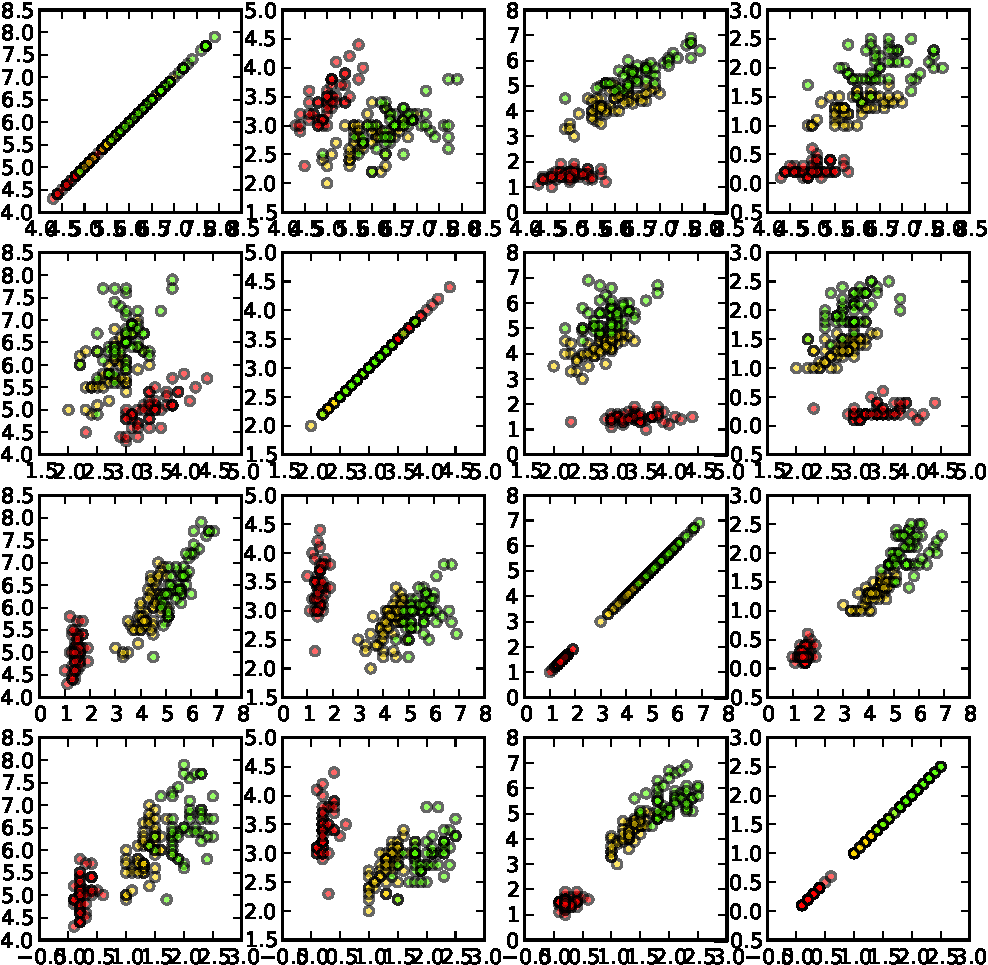
\includegraphics[height=.99\textheight]{pca-pics/iris-all}

  \end{center}
\end{frame}

\begin{frame}
  \frametitle{Plotting the Data}
  \begin{columns}
    \column{.5\linewidth}

    \begin{enumerate}
    \item<1-> Which one of those projections is \alert{good}?
    \item<2-> Are there others, possibly \alert{better} projections?
    \item<3-> \alert{Which variables} are involved in the best
      projections?
    \end{enumerate}
    \column{.5\linewidth}
    \includegraphics<1->[width=\linewidth]{pca-pics/iris-all}
  \end{columns}
\end{frame}

\begin{frame}[fragile]
  \frametitle{Principal Component Analysis}
  \begin{itemize}
  \item PCA projects to axis with greatest \alert{variance}
  \item Often provides good \alert{first insight} into dataset
  \end{itemize}

  \begin{columns}
    \column{.5\linewidth}
    \begin{lstlisting}[escapechar=!]
      P !$\leftarrow$! PCA(X, 2)
      X2 !$\leftarrow$! P * X'
    \end{lstlisting}
    \column{.5\linewidth}
    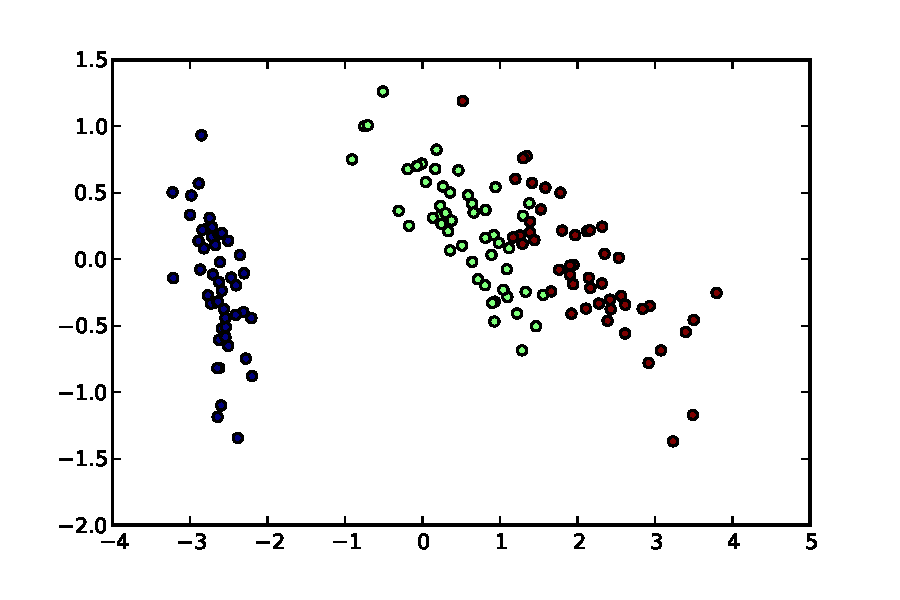
\includegraphics[width=.99\linewidth]{pca-pics/iris-2d}
  \end{columns}

  \pause
  \begin{itemize}
  \item Important variables: Take a look at the projection matrix \verb+P+:
  \end{itemize}

  \begin{lstlisting}[escapechar=!]
    P = [[ 0.36 -0.08 !\alert<3>{0.85}! 0.35]
         [!\alert<4>{-0.65}! !\alert<4>{-0.72}  0.17  0.07]]
  \end{lstlisting}
\end{frame}

\begin{frame}
  \frametitle{Noise Reduction}
  \begin{itemize}
  \item Most of the data explained by first axes
  \item (almost) constant axes thrown away
  \item Projecting back to input-space reduces noise
  \end{itemize}
  \begin{center}
    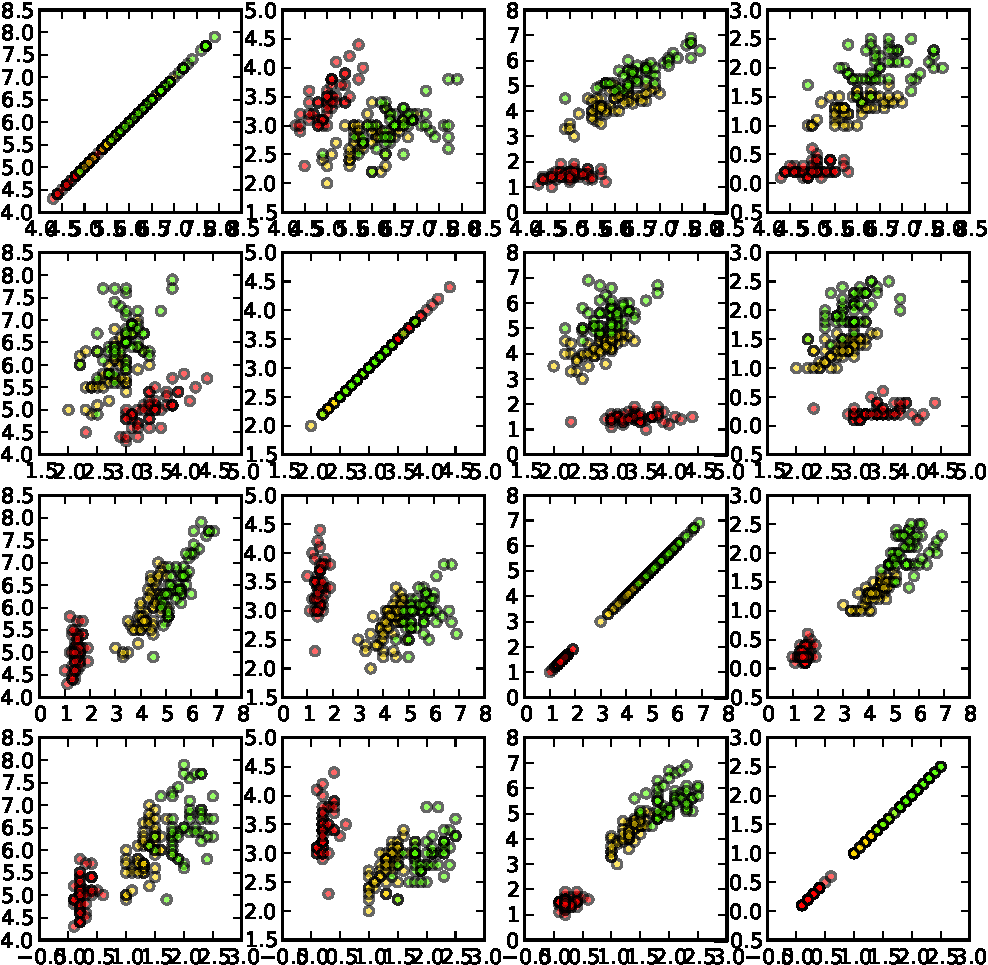
\includegraphics[width=.47\linewidth]{pca-pics/iris-all}\hfill%
    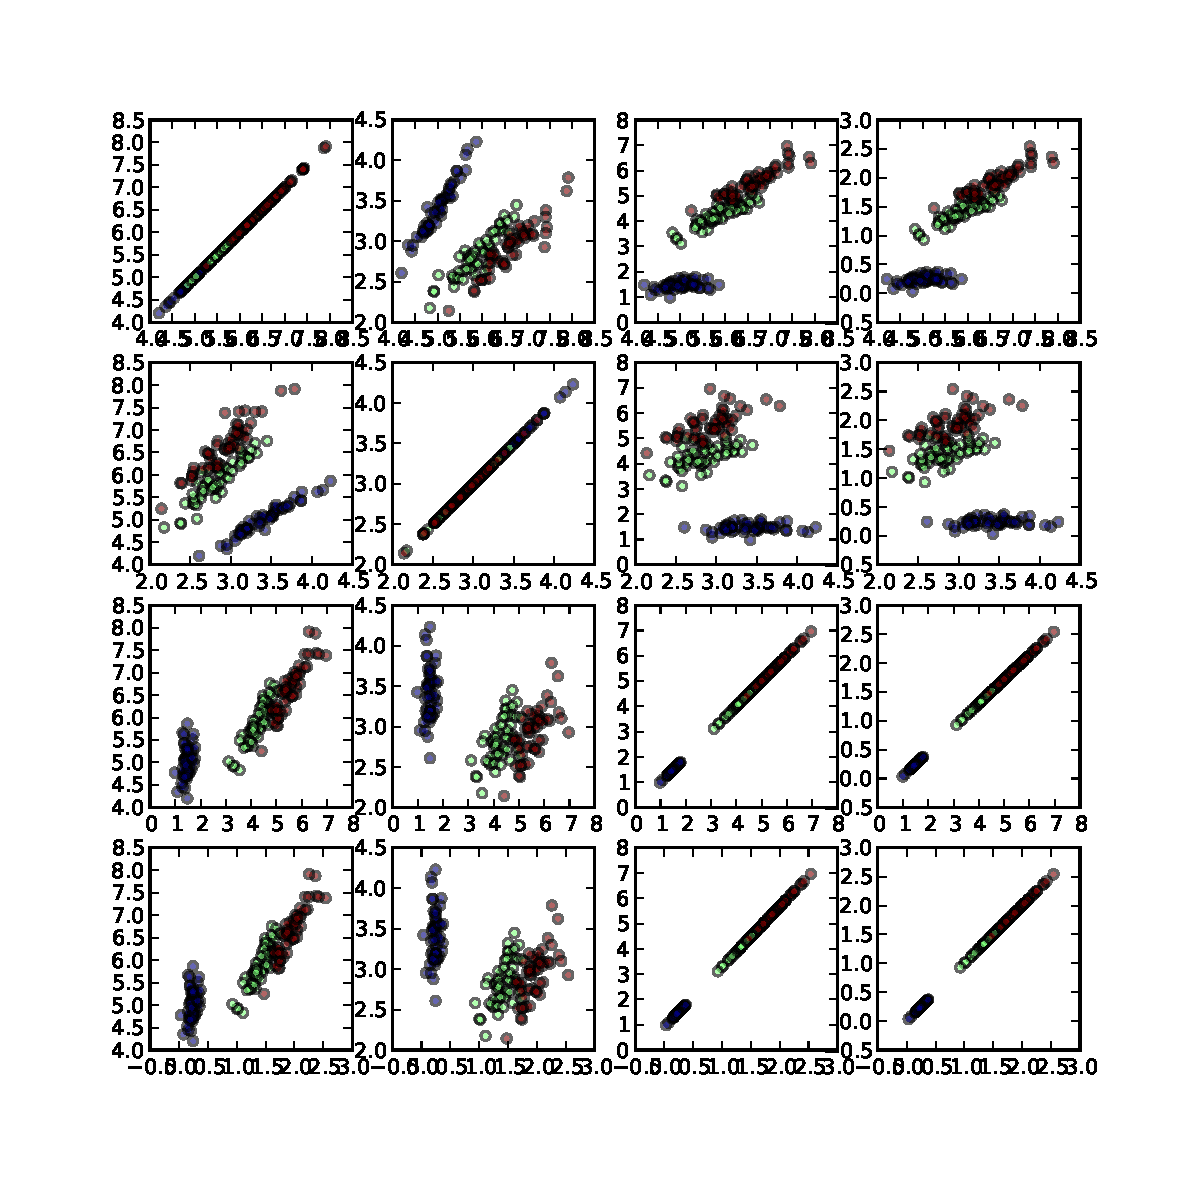
\includegraphics[width=.47\linewidth]{pca-pics/iris-bt}
  \end{center}
\end{frame}


